\documentclass[12pt,a4paper]{report}

\usepackage{dolgozat}

\usepackage{hyperref}

\usepackage{listings}
\usepackage{cpp}
\usepackage{java}
\usepackage{python}

\linespread{1.2}

\begin{document}

\pagestyle{empty} %a címlapon ne legyen semmi=empty, azaz nincs fejléc és lábléc

\begin{flushleft}
\textsc{\bfseries Miskolci Egyetem}\\
Gépészmérnöki és Informatikai Kar\\
Alkalmazott Matematikai Intézeti Tanszék
\end{flushleft}

%A fõiskola logoja
{\large
\begin{center}
\vglue 1truecm
\textbf{\huge\textsc{Szakdolgozat}}\\
\vglue 1truecm

\epsfig{file=cimlap/ME_logo.eps, width=4.8truecm, height=4truecm}\\
\textbf{\textsc{Miskolci Egyetem}}
\end{center}}

\vglue 1.5truecm %függõleges helykihagyás

%A szakdolgozat címe, akár több sorban is
{\LARGE
\begin{center}
\textbf{Programozási nyelv magas szinten átvihető alkalmazások fejlesztéséhez}
\end{center}}

\vspace*{2.5truecm}
%A hallgató neve, évfolyam, szak(ok), a konzulens(ek) neve
{\large
\begin{center}
\begin{tabular}{c}
\textbf{Készítette:}\\
Horváth Máté János\\
Mérnökinformatikus BSc
\end{tabular}
\end{center}
\begin{center}
\begin{tabular}{c}
\textbf{Témavezető:}\\
Piller Imre, egyetemi tanársegéd
\end{tabular}
\end{center}}
\vfill
%Keltezés: Hely és év
{\large
\begin{center}
\textbf{\textsc{Miskolc, 2018}}
\end{center}}

\newpage


\cleardoublepage
\pagenumbering{gobble}
\tableofcontents
\cleardoublepage
\pagenumbering{arabic}

\newpage

\pagestyle{fancy}

\Chapter{Bevezetés}

A dolgozat egy olyan magas szintű programozási nyelv definiálását tűzi ki célul, mely fordítás után más, magas szintű programozási nyelvre fordul le. Ennek segítségével a programkódot nagyon könnyen lehet egyidejűleg több platformra is akár elkészíteni, hiszen a program egy adott nyelven történő megírása után a fordítás során több nyelvre, több platfomra lehet fordítani.
A dolgozat elkészítése során fontos szempont volt megvizsgálni a célnyelvkent elérni kívánt programozási nyelveket, azok szintaxisát, azokat összehasonlítani, hogy a hasonlóságok és különbségek kiemelése révén megfogalmazható legyen, hogy milyen legyen a definiált nyelv.
Emellett mindenképpen vizsgálni kellett a programkód feldolgozásának lépéseit, a parser és lexer működését. A következő lépés pedig az eddig megszerzett ismereteit alapján az elkészíteni kívánt nyelv tulajdonságait, vezérlési szerkezeteit, definiálni az elemeit.
\Chapter{Keresztfordítás}

\section{Formális nyelvek}

A formális nyelvek bevezetéséhez először is át kell tekintetni, az ábécé, a nyelv és nyelvtan fogalmát.

"Szimbólumok tetszőleges nemüres, véges halmazát ábécének nevezzük és V-vel jelöljük." (Dömösi Pál, Falucskai János, Horváth Géza, Mecsei Zoltán, Nagy Benedek - Formális Nyelvek és Automaták https://gyires.inf.unideb.hu/KMITT/b24/) Látható tehát, hogy az ábécét egy halmazként definiáljuk, mely nem üres halmaz és tetszőleges szimbólumokat tartalmaz. Bár az említett könyvben a definíció szerint V-vel jelölik az ábécét, általánosságban azt mondhatjuk, hogy nagybetűvel (A, B) esetleg $\Sigma$ karakterrel történik ennek jelölése.

"A V ábécé feletti szavak egy tetszőleges L halmazát a V ábécéből alkotott (formális) nyelvnek nevezzük" (Dömösi Pál, Falucskai János, Horváth Géza, Mecsei Zoltán, Nagy Benedek - Formális Nyelvek és Automaták https://gyires.inf.unideb.hu/KMITT/b24/), azaz a nyelv egy az adott ábécé felett értelmezett szavak tetszőleges halmaza lesz. Általánosan formális nyelveknek nevezünk minden olyan nyelvet, melyekben véges hosszúságú szavak generálhatók véges ábécékből. A programozási nyelvek alapvetően ilyen formális nyelvek.

Az informatikához kapcsolódóan az ilyen leírást a formális nyelvtannal jellemezzük, mely konkrétan egy formális nyelvet ír le.

A nyelvtan két nagy kategóriája a generatív és analitikus nyelvtan. Előbbi azt írja le, hogyan lehet előállítani az adott nyelvet egy adott szabályhalmazból, míg utóbbi az adott nyelv olvasását írja le, ugyancsak szabályokkal.
A generatív nyelvek tekintetében meg kell említeni azok osztályozását is. Ezt először az 1950-es években vetette fel Noam Chomsky nyelvész, mely osztályozást róla nevezték Chomsky-hierarchiának.

"Chomsky négy nyelvosztályt definiált. Ezeket számokkal jelölte, így van 0-ás, 1-es, 2-es és 3-as nyelvosztály. Az egyes nyelvosztályokban a helyettesítési szabályok alakjára vonatkozóan Chomsky az osztály sorszámának növekedésével egyre szigorúbb megkötéseket írt elő." (BACH IVÁN - Formális nyelvek https://www.typotex.hu/download/formalisnyelvek.pdf)

 Ez a besorolás 4 osztályba sorolja a nyelveket az alapján, hogy mennyire kifejezőek, illetve milyen szigorú megkötések vonatkoznak rájuk. Az alábbi táblázatban lehet összefoglalni az egyes csoportokat, azaz osztályok tulajdonságait.
 
\begin{table}
	\caption{Chomsky-hierarchia}
	\label{1. táblázat}
	\begin{tabular}{c|c|c|c|c}
		\textbf{Nyelvoszály} & \textbf{Nyelvtanok} & \textbf{Nyelvek} & \textbf{Automaták} & \textbf{Produkciók szabályok}\\
		0. nyelvosztály & Rekurzívan megszámlálható & Rekurzívan megszámlálható & Turing-gép & Nincs megkötés\\
		1. nyelvosztály & Környezetfüggő & Környezetfüggő & Korlátos nem determinisztikus Turing-gép & $\alpha$A$\beta$ -> $\alpha$$\gamma$$\beta$\\
		2. nyelvosztály & Környezetfüggetlen & Környezetfüggetlen & Nem determinisztikus veremautomata & A -> $\gamma$\\
		3. nyelvosztály & Szabályos & Szabályos & Véges determinisztikus automata & A -> a illetve A -> aB vagy A -> Ba\\
	\end{tabular}
\end{table}
(Formális nyelvtan - https://hu.wikipedia.org/wiki/Formális\_nyelvtan)

A hierarchia 3. nyelvosztályába tehát olyan nyelvtanok tartoznak, melyek bal oldal mindig egy nemterminális szimbólum, a jobb oldala pedig vagy egy nemterminális szimbólum, vagy egy terminális és nemterminális szimbólum által alkotott sor.

A 2 nyelvosztályban található nyelvtanok szabály szerint az A -> $\gamma$, ahol a $\gamma$ tetszőleges jelsorozat, mely terminális és nemterminális szimbólumokat is tartalmazhat. Az A pedig egy itt is egy nemterminális szimbólum lesz.

Az 1. nyelvosztályt a környezetfüggő nyelvek osztályának nevezzük, ezt mutatja a szabály is, az $\alpha$A$\beta$ -> $\alpha$$\gamma$$\beta$, azaz a leírás szabálya a A ->$\gamma$, de ez csak az $\alpha$ - $\beta$ környezetben alkalmazható.

A 0. nyelvosztály tekintetében ilyen megkötés nincs, mint ahogy azt a fenti táblázat mutatja.

\subsection{Véges automaták}

Fontos szót ejteni a véges automatákról (Final State Automata, FSA). A véges automaták olyan automaták, melyek meghatározott véges állapothalmaz, bemeneti ábécé, kezdő és végállapot valamint átmeneti függvény megadása után egy rendszert képez. Ez felírható egy irányított gráffal, itt az egyes állapotok a gráf csúcspontjai. Mivel véges automatáról van szó, az automata az egyik állapotból egy input hatására egy másik állapotba kerül.

Két nagy csoportot különböztetünk, a determinisztikus és a nem determinisztikus automata. A nem determinisztikus automata esetében lehetnek olyan szavak, melyeket nem tud beolvasni, mivel egyes átmeneteknél elakadhat. Viszont a nem determinisztikus automata egy adott input szimbólum hatására egy adott állapotból több állapotba is átmehet. Véges automaták felhasználhatók a reguláris nyelvek leírására.

% TODO: Itt elég csak a determinisztikus véges automatákra koncentrálni!

\subsection{Reguláris nyelvek}

A reguláris nyelvek reguláris kifejezések segítségével kifejezett formális nyelv, melyeket a véges automaták képesek felismerni és értelmezni. Reguláris kifejezéseket több helyen is használnak az informatikában, mivel többféle kifejezést is értelmezni lehet, illetve sok helyen ellenőrzéseket lehet velük végezni különféle adatokon.

A reguláris nyelvek pedig a különféle programozási nyelvek feldolgozásánál nyújtanak segítséget, a lexer és parser generátorok egyes elemeinél, melyek alapján a generátorok készítése megtörténik.

A fenti elemek készítése során a reguláris nyelvek használata végett mindenképpen meg kell vizsgálnunk a leíráshoz használt jelölésrendszert. Ilyen esetben az Extended Backus-Naur Form (ENBF) és railroad, vagy szintaxis diagram segítségével tudjuk a megfelelő nyelvtant összeállítani.

\subsection{Extended Backus-Naur From}

A Backus-Naur Form egy formális nyelvek leírására használható metanyelv, melyet John Backus hozott létre és mutatott be. Maga a metanyelv valójában szabályok halmaza, melyben terminális és nemterminális elemek találhatók meg adott összerendelésben, azaz kifejezésben melynek bal és jobb oldalán egy-egy elem áll általában ::= vagy : jellel összekapcsolva ;-vel lezárva a kifejezést.

A terminális elemek olyan nyelvi elemek, melyek előre definiáltak, mint például a literálok (string literál, integer interál). A terminális elemeket a fentebb említett kifejezések bal oldalán nem jelennek meg.
A nem terminális kifejezések ezekből a terminális kifejezésekből, más nemterminális kifejezésekből, vagy ezek kapcsolataiból állnak.

id ::= 	STRING
	;
integer ::= INT
	;

Az fentebb látható esetekben a kifejezések bal oldalán egy-egy nemterminális kifejezés áll, a jobb oldalon ezzel szemben terminális kifejezés, string, illetve integer literál áll. Az alább látható kifejezésben ezután felhasználhatjuk a már definiált elemeket is.

sum ::=	integer "+" integer
	;

Megadhatók a kifejezések olyan módon is, hogy egy bal oldalon álló nemterminális kifejezés több módon is előállítható. Ilyenkor a jobb oldalon álló kifejezéseket | jellel, azaz vagy kapcsolattal kell elválasztani. Emellett megadható benne ""-ek között álló konkrét string is.

sum ::= integer "+" integer
	;
neg ::= integer "-" integer
	;
	
mul ::= integer "*" integer
	;

summul ::= "(" integer + integer ")" * integer

count ::= sum 
	| neg
	| mul
	| summul
	;
	
Az Extended Backus-Naur Form (EBNF) ennek a BNF-nek egy kiterjesztése. Ebben a formális nyelv még pontosabb leírását segítő elemek jelentek meg, melyek közül a legfontosabbakat említjük itt meg.

A nyelv leírásában használhatjuk a [ kifejezes ] alakot, mely esetben a szögletes zárójelpárba írt kifejezések opcionálisak, nem kötelezően megjelenő elemek a szabályok alkalmazásakor.
Lehetőségünk van jelezni, hogy egy adott szerkezetben egy vagy több elem ismétlődhet. Ezt a { elem } kifejezéssel tehetjük meg, mely jelentése az adott elem nulla vagy többszöri megjelenése.
Emellett a zárójelpárba írt elemek csoportosíthatók azaz jelölhető például egy adott szabályban, hogy több különféle kifejezésre illeszkedhet.

math ::= integer ("+" | "-" | "*" | "/" ) integer

A fenti példában tehát a szabály olyan esetekre illeszkedik amikor két integer jelenik meg, viszont a közöttük lévő jel a +, a -, a * és a / bármelyike lehet.

http://matt.might.net/articles/grammars-bnf-ebnf/

% TODO: Railroad/szintaxis diagramok (Pl.: JSON.org, SQLite dokumentáció)

\section{A feldolgozás lépései}

A \aref{fig:process}. ábrán láthatóak a fordítás legfőbb lépési, a következőkben ezeket nézzük át röviden.

\begin{figure}
\centering
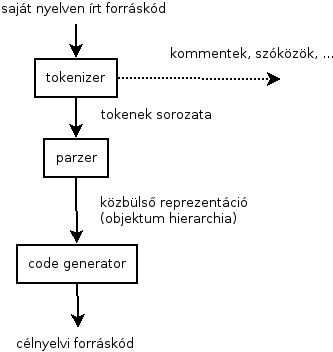
\includegraphics[scale=1]{kepek/process.png}
\caption{A keresztfordítás lépései}
\label{fig:process}
\end{figure}

\subsection{Tokenizálás}

Az tokenizálás a fordítás első lépése lesz, ebben a lépésben a felhasználó által megadott programkód beolvasásra kerül, majd a program szétbontja azt és megvizsgálja az egyes elemeket. A tokenizer minden elemhez hozzá kell tudjon rendelni a program egy tokent, így a tokenizer visszatérési értéke tokenek egy sorozata lesz.

A tokenek sorozatában nem szerepelnek a különböző fehér karakterek, mint a szóköz, újsor, tabulátor karakter, mivel a tokenizer a feldolgozás során ezeket az elemeket, mivel ezek csak az olvashatóságot növelik a kódban, a feldolgozásához, fordításhoz plusz információval nem járulnak hozzá, törli.

Ezután a többi tokent a megadott reguláris kifejezések alapján hozza létre. A leggyakoribb tokenek közül néhány példa:
szám literál: \texttt{[0-9\_]+}
szöveg literál: \texttt{[a-zA-Z0-9\_]+}
zárójelek: \texttt{(} és \texttt{)}
fehér karakterek:
\begin{verbatim}
(\\n | \\r | \\r\\n | \\f | \\t)+
\end{verbatim}

A tokenizer általában egy külön programrész, osztály a feldolgozóban, melyet általában lexernek is neveznek. Ezt az osztályt külön programok segítségével lehet megalkotni, melyeket lexer generatornak nevezik. Az interneten többféle ilyen generátor is található, melyeket segítségül hívva meg lehet alkotni a feldolgozó osztályt.

Fontos, hogy ezeknek a generátoroknak meg kell adni egy szintaktikai leírást, mely alapján a lexert létrehozzák, azonban figyelni kell arra, hogy az adott generátornak megfelelő módon, és a általunk megadott nyelvre illeszkedő kifejezéseket adjunk meg.

A fellelhető generátorok közül jelen esetben olyanok közül kell választani amelyek a reguláris kifejezések segítségével adják meg a feldolgozási elemeket. Ilyenek  például az AnnoFlex, JFlex programok, ezekről részletesebben a szintaktikai elemzés fejezetben esik szó.

A megvalósításkor nehézséget okozott a fentebb említett választás és szintaktikai leírás. Mivel a korábbi tanulmányaim során ilyenre nem került sor, a generátor általt felhasznált szintaktikai leírás megvalósítása néhány esetben hibára futott. Ami ebben segítséget jelentett, az az AnnoFlex programban megadott példa kód volt, mely alapján további reguláris kifejezéseket fel lehetett venni.

\subsection{Parser}

A tokenek sorozata ezután átkerül a feldolgozás következő lépéseként a parserhez. A parser osztályt, mely a kapott kódot feldolgozza, szintén előtte definiálni kell, melyet az adott nyelvhez kapcsolódó megadott szintaktika, illetve egy parser generator végezhet el.

A lexer generatorthoz hasonlóan a parser generator is megtalálható az interneten. Fontos megjegyezni, hogy olyan parser és lexer generatort érdemes választani, mely a lehető legjobban együtt tud műküdik. Ilyen például a JFlex és a CUP generátor, mely generátort úgy terveztek, hogy egymással együttműködve tudnak működik.

A CUP generátort emellett magában is használható egy adott token sorozat feldolgozására, ezekről részletesebben szintén a szintaktikai elemzés fejezetben esik szó.

Szintén nehézséget okozott a megfelelő parser generátor kiválasztása, hiszen annak olyannak kell lennie, hogy a kiválasztott lexer generátorral együtt tudjon működni, az az által generált eredményhalmazt be tudja olvasni. Itt is felmerültek a fájl szintaktikai megvalósításakor fellépő hibák. Sajnos a CUP parser generátor leírása nem volt annyira részletes ez ügyben, így a hibák javítása hosszabb időt vett igénybe.

\subsection{Kód generálás}

Az utolsó lépés, hogy miután a parser generator által létrehozott objektum hierarchia elkészült, ebből a program elvégzi a konvertálást, és gíy jön létre majd a célnyelvi forráskód, ami már az adott nyelv szintaktikájának megfelelő és felhasználható a programozó izlése szerint.

\Chapter{A nyelv definíciója}

\section{Általános szempontok}

A saját nyelv kialakításánál az elsődleges szempont a könnyű kezelhetőség volt, hogy bár több nyelvre, több platformra kerülhet lefordításra a kód, a felhasználó, programozó egyszerűen, könnyen tudja megírni a kódot a definiált nyelven, így nem kell minden célnyelvi szintaktikai és szemantikai szabállyal tisztába lennie, azokat külön-külön alkalmaznia.

Ezek alapján a nyelv a Python nyelvhez hasonló megoldásokat és jegyeket hordoz magán, a nyelvi szintaktika és szemantika megvalósításának tekintetében.

Ahhoz, hogy a nyelvet definiálni lehessen az alábbiakban áttekintjük a feladat során célnyelvként tekintett nyelveket általánosan, azok megvalósítását, tulajdonságait, fő elemeit. Majd ezután a saját definiált nyelv tervezett nyelvi elemeit vesszük sorra.

\section{A célnyelvek áttekintése}

A dolgozat szempontjából célnyelvnek azon magasszintű programozási nyelveket tekintjük, melyekre a felhasználó által, a definiált nyelven írt kód a program futtatásának végén lefordul. A program jelenleg nem minden magasszintű programozási nyelvre képes fordítani, tehát nem minden magasszintű programozási nyelv tekinthető célnyelvnek, valamint jelenleg a célnyelvként tekintett magasszintű nyelvek nem minden nyelvi elemét támogatja a program. Ezek a program egy későbbi fejlesztése során elérhetővé válhatnak. Az alábbiakban a dolgozat szempontjából tekintett célnyelveket vizsgáljuk meg röviden.

\subsection{C}

A C nyelv magasszintű, általános célú programozási nyelv, mely az egyik legelterjedtebb programozási nyelv, a ma fellehető számítógép architektúrák szinte mindegyikére készült C fordító. A nyelv sturkturált és szabványos programozási nyelv, ugyanúgy megtalálhatóak itt a vezérlési szerkezetek mint a többi magas szintű nyelvben. Változó deklarálásakor meg kell adni a változó nevét és típusát is, mivel a nyelv erősen típusok nyelv. A változó neve konvenció alapján betűvel kezdődik és utána betűket és számokat tartalmazhat. Ezután egyenlőségjellel adhatjuk meg a változó értékét. C nyelven az utasításokat a sor végén ;-vel zárjuk le. Mivel az egyes utasítások lezárását ; jelzi, a nyelven a sortörések kihagyhatók, ezek a fehér karakterek csak az olvashatóságot növelik, a fordítás során eltávolítására kerülnek. C nyelven írt programok során is az utasítások szekvenciálisan futnak le.

A nyelv nem objektum orientált nyelv, azaz osztályok definíció szintjén nincsenek a nyelvben. Jelen dolgozat további nyelveiben megjelenik ez a funkció, osztályba szervezhető a kód, csakúgy mint a definiált nyelvben is, így valamivel nehezebb C módra történő fordítás. C nyelven a struktúrák találhatók meg, melyek a typedef struct kulcsszóval vezethetnek be. Ebben adhatók meg az osztályokhoz hasonló programelemek. Szintén fontos különbség, hogy a C nyelven megjelennek a pointerek, melyek egy adott változó címere mutató változók. Ezáltal érték szerint és cím szerint is át lehet adni változókat.

C nyelven emellett használható a szelekció, azaz az elágazás. Ezt az if kulcsszó vezeti be, ami után ( és ) között kell megadni az elágazás feltétet. Itt a rendszer azt vizsgálja a megadott feltételek igaz vagy hamis, és aszerint fut le az adott ágban megírt kód. A szelekció többi ágat az else if (feltétel) és az else kulcsszó vezeti be. A C nyelv is ismerni a switch szelekciót, itt is meg kell adni egy kifejezést, változott és a switch belül megadni azon kifejezéseket melyekre az illeszkedést a program vizsgálni fogja.

Emellett a programban megadható iteráció is. Ciklusból a nyelven 3 különböző van, a while, for és do while. Ezek mindegyikéhez kell egy ciklusváltozó, egy feltétel, melyet minden egy ciklusban ellenőriz a rendszer. A for és a while elöl tesztelő ciklus, míg a do while hátul tesztelő, azaz az egyszer biztos le fog futni a cilkusmag, míg az előző kettőben nem biztos. A C nyelvben nincs külön hibakezelés, minden ilyen feladatot a programozónak kell feltételvizsgálattal megoldania, illetve klasszikus esetben nincs automatikus szemétgyűjtő algoritmus sem, a memória felszabadításáról is a programozónak kell gondoskodnia.

\subsection{JavaScript}

A JavaScript egy scriptnyelv, mely leggyakrabban a böngészőben jelenik meg, és kliens oldalon is látható a kódja. A nyelv először MochaScript néven lett létrehozva, majd később a szintaxisa a Java nyelvhez lett hasonló, itt lett a neve JavaScript.

A nyelvet a böngészőkben használt html nyelv statikusságának megtörésére használták, illetve JavaScript segítségével egyszerűen elvégezhető előzetes ellenőrzés az adatokra, mely mellett azonban természetesen mindenképpen kell szerver oldali ellenőrzés is, mivel ahogyan fentebb említettem a JavaScript kód látható böngészőben is különféle eszközökkel, így akár manipulálható is. A kódot a html kódba is ágyazhatjuk, de legtöbbször egy külön .js fáljban van elhelyezve. A JavaScript gyengén típusos nyelv, a változók definiálásakor nem kell típust megjelölni. A változó értéke fogja megadni a változó típusát.

A JavaScriptben is megtalálhatók az ismert vezérlési szerkezetek, ugyanúgy használható az értékadás, szekvencia, szelekció és iteráció is. Sőt még objektum orientálttá is tehető a nyelv. A JavaScriptben külön kifejezéssel lehet változót deklarálni, ez a var kulcsszó, melyet mindig meg kell adni, ezután következik a változó név majd az érték.

Külön meg kell említeni a láthatóságot a JavaScript esetében. Itt a változók alapértelmezetten csak az adott scope-ban elérhetők, ahol létre lettek hozva. Általános esetben mindenképpen egy függvény kerül megírásra, és ebben történik a változók létrehozása, a műveletek elvégzése. A változók csak az adott függvényen belül láthatók ahol létre lettek hozva. Megadhatók azonban olyan módon is a változók, hogy máshonnan is elérhető legyenek, ekkor a függvényen kívül kell deklarálni őket, így globális változókká válnak és elérhetők. Másik módszer ha olyan változóknak adunk értéket amik még nincsenek is deklarálva. A JavaScript ebben az esetben létrehozza a változót, mely azonban globális változóként kerül létrehozásra.

Fentebb említettem a JavaScriptet, mint objektum orientálttá tehető nyelvet. A JavaScriptben általánosságban mindig egy függvényt írunk a function kulcsszóval, még akkor is, ha ez esetleg rejtetten, mondjuk egy jQuery fájlban az alábbi módon nézne ki:

\begin{cpp}
$("data").click(function() {
	utasitasok;
});
\end{cpp}
% $

Látható a fentebbi kódban is megjelenik a function kulcsszó. A nyelv objetum orientáltsága mindössze annyit jelent, hogy egy osztályként használt függvényt írunk meg, majd ennek adunk adattagokat és további függvényeket is, és végül ezt fogjuk használni objektumként, azaz osztályként.

A JavaScript esetében minden utasítássort \texttt{;}-vel kell lezárni szintaktikailag, tehát ebben hasonlít az általánosan vizsgált programozási nyelvekhez.

\subsection{Python}

A Pyhton egy objektum orientált programozási nyelv, mely egyre nagyobb teret hódít egyszerű kezelhetősége és rugalmassága miatt. Guido van Rossum a nyelv megalkotásakor a fent emlíett egyszerűséget tartotta a legfontosabbnak.

A nyelv gyengén típusos nyelv, tehát itt sem kell megadni típusmegjelölést, illetve fontos különbség a többi nyelvhez képest, hogy nem használnak \texttt{;}-t az utasítások lezárásakor, így az utasítások végét a sor vége jelenti. Más magas szintű nyelvekkel ellentétben itt ezért nem is lehetne az egész kódot egy sorban megadni.

Emellett szintén fontos különbség a blokkokat jelző \texttt{\{} és \texttt{\}} hiánya, a nyelv az olvashatóságot is segítendő, a tabulátorokkal történő behúzással jelzi az egyes blokkokat.

Általánosságban egy adott metódus, osztálydefiníció, elágazás, megírásakor a sor végére \texttt{:}-ot teszünk, ezután a következő sortól tabulátor behízással történik az adott feltétel vagy osztály magjának leírása.

A nyelv támogatja az objektum orientált leírást, a class kulcsszóval bevezetett osztályokat lehet megírni, melyben definiálhatunk változókat, metódusokat majd példányosíthatjuk csak úgy mint az általánosságban vizsgált programozási nyelvek esetében.

\subsection{PHP}

A PHP egy szerveroldali nyelv, tulajdonképpen scriptnyelv, az így megírt fájlok futtatásához a fizikai szervergépre valamilyen PHP fordítót kell telepíteni és konfigurálni. Legelterjedtebb manapság még mindig az Apache webszerver, mely a UNIX rendszerekre telepíthető.

Érdemes kiemelni a PHP hiba, illetve figyelmeztetés kijelzését is, mely szerver oldalon, az Apache konfigurációs fáljában, illetve a PHP fájlban is letiltható, illetve engedélyezhető. Érdemes ezt mindig engedélyezni a fejlesztés során, mivel egyéb esetben egyes hibák elfedésre kerülnek a PHP rugalmassága miatt, így a végső eredmény is hibás lehet. Például az alábbi kódban:

\begin{cpp}
<?php
   function multiply ($value) {
      $value = $value * 10;
      return $value;
   }
   
   $retval = multiply();
   Print "Return value is $retval\n";
?>
\end{cpp}

Látható, hogy a multiply függvény egy paramétert vár, és azzal számol, azonban a meghívásakor nem kerül átadásra paraméter. Ilyenkor a PHP rugalmassága miatt, egyszerűen 0 értékkel fog számolni a program, azaz a végeredmény is nulla lesz.

Azonban ez nyilvánvalóan nem a helyes működés lenne (kivéve természetesen, ha pont a 0 számmal szeretnénk meghívni egyébként is a metódust), ezért érdemes bekapcsolni a hibajelzést. Ilyenkor a program kijelzi, hogy bár a metódus deklarálásakor megadtuk, hogy paramétert várunk, meghívásakor nem adtunk neki paramétert.

Általánosságban a PHP megvalósítása miatt, ha ilyen hibákat vétünk (és ha nincs hiba kijelzés) a PHP mindig megpróbálja megoldani, a programot lefuttatni.

A PHP alapvetően nem objektum orientált nyelv. Eredetileg ez szerveroldali scriptnyelv volt, csak a 2004-ben kiadott 5-ös verzióval került be az objektum orientáltság. Mivel a PHP akkoriban a legnépszerűbb szerveroldali scriptnyelv volt, sőt még manapság is az, nagyon sok olyan kód készült, melyben objektum orientált leírás nem volt, így ezeket először át kellene alakítani objektum orientálttá.

\subsection{Java}

A Java nyelven megírt kódok futtatásához is saját környezet kell. A java telepíthető minden operációs rendszerre, valamint komplexitása miatt az egyik legelterjedtebb és leginkább használt nyelv.

A Java nyelvben, ha bármilyen hibát vétünk akkor már a kód fordítása során erről értesítést kapunk, a fordítás pedig leáll. Tehát Java nyelvben a fenti kód (itt természetesen osztályt is kell definiálnunk, majd annak a metódusát meghívni):

\begin{lstlisting}[language=Java]
public class Test {
    private value;
    
    Test(int value) {
        this.value = value;
    }

   public void multiply() {
      value = value * 10;
      System.out.println("Return value is: " + value);
   }

   public static void main(String args[]) {
      Test test = new Test();
      test.multiply();
   }
}
\end{lstlisting}

Ez a kód már fordításkor hibát fog jelezni, hiszen a konstruktorban zárójelpárban megadtuk, hogy várunk egy integer értéket, viszont a main függvényben az osztály inicializálásakor nem adtunk meg értéket. 

\section{Saját nyelvi elemek}
A saját nyelv definiálásakor a fentiek alapján az alábbi nyelvi szintaktika kerül kialakításra.
A definiált nyelvben is a megadott konstrukciók végrehajtási sorrendjét a vezérlési szerkezetekkel szabályozhatjuk, melyek az értékadásokon kívül a szekvencia, szelekció és iteráció.

A nyelvben az értékadás a Python nyelv egyszerűségét idézi, azaz meg kell adni egy változó nevét és az értékét. Ahogy az utasítások sorának végére, ide sem kell ;-t tenni.

Az értékadást az alábbi példa szemlélteti:
\begin{cpp}
string szoveg = "szoveg"
\end{cpp}

A változók definiálásakor meg kell adni a változó típusát, mivel a nyelv erősen típusos. A nyelv az int, string, double, boolean, void, array és dictionary típusokat ismeri, melyek minden tekintett célnyelvben megtalálhatók, a C nyelvben a string karaktertömbként, illetve a dictionary struktúraként, így mindegyik nyelvre lehet fordítani.

\begin{cpp}
int valtozo1 = 5 ~ szám típusú
string valtozo2 = "szöveg" ~ text/string tipusú
string valtozo3 = valtozo1 + valtozo2 ~ eredmény 5szöveg, mint string típusú változó
\end{cpp}

A változók, illetve osztály adattagok esetében meg lehet adni láthatósági módosítót is, azonban ez nem kötelező. Ha nincs megadva láthatósági módosító egy adott változóhoz, akkor a nyelvi definicíó alapján alapértelmezetten private láthatóságú lesz a változó, azaz csak az adott osztály, amiben a változó létre lett hozva, az tudja majd kezelni, kívülről nem lehet.

Ha azt szeretnénk, hogy kívülről is lehessen kezelni az adott változót, akkor mindenképpen ki kell írni a láthatósági módosítót. Ilyen esetben public módosítót kell megadni, így mindenhonnan elérhető az adott változó. A metódusok belül létrehozott változók minden esetben a metódusokon belül használhatók.

array valtozoT = {1, 2, 3, 5, "tizenkettő"} ~ egy adott tömbben többféle típusú elem is szerepelhet, például szám és szöveg. A tömb elemeire a valtozoT(x)-el lehet hivatkozni, ahol az x a tömb x. eleme lesz.
Túlindexelés esetén a porogramozónak figyelnie kell, ugyanis a nyelv rugalmassága miatt nem fog hibaüzenetet kapni. Ha a tömb 10 elemű és a tomb(12)-t hívjuk akkor a változóba ahol az elemet letároljuk, vagy metódusba ahova átadjuk egy 0 kerül át.

\begin{cpp}
array tomb = valtozoT + "húsz"
Print(tomb) ~ eredmény: 1 2 3 5 tizenkettő húsz
Del(tomb)
array tomb = valtozoT
tomb(2) = 1.25
tomb(3) *= 5
Print(tomb) ~ eredmény: 1 1.25 15 5 tizenkettő
Del(tomb)
array tomb = valtozoT
Print(tomb(7)) ~ eredmény: 0
Del(tomb)

array tomb = valtozoT + {5, "nyolc", "miskolc"} ~a már letárolt, névvel ellátott tömbhöz egy névtelen tömböt fűzünk hozzá, ez önmagában nem tárolódik a memóriában, csak az új változóban az eredeti tömbbel együtt, ahhoz hozzáfűzve
valtozoT += {5, "nyolc", "miskolc"} ~ ugyanaz mint az előbb, csak itt nem jön létre új változó, a már meglévőhöz kapcsolódnak az új elemek
Print(tomb) ~ eredmény: 1 2 3 5 tizenkettő 5 nyolc miskolc
Print(valtozoT) ~ eredmény: 1 2 3 5 tizenkettő 5 nyolc miskolc
\end{cpp}

A második vezérlési szerkezet az elágazás. A definiált nyelvben a szelekció az If kulcsszóval kerül bevezetésre, melyet egy feltétel követ. A feltétel három tagból kell, hogy álljon, mely egy operátor és annak két oldalán valamilyen kifejezés kell, hogy legyen.

Az elágazás további ágait ElIf kulcsszóval vezetjük be, mely után szintén egy feltétel kell, hogy álljon, melynek a szerkezete az If feltételével megegyező kell, hogy legyen. Illetve egy utolsó ág van fenntartva arra az esetre, hogy ha a szelekció egyik korába ágának feltétele sem teljesül ezt az Else kulcsszóval kell bevezetni, itt nem kell feltételt megadni.

A szelekció egyes ágain több végrehajtható művelet is helyet kaphat, melyeket a program sorrendben, szekvencia alapján végez el. Az egy adott ághoz tartozó műveleti blokkot a programnyelvben nem kell külön zárójel, illetve kapcsos zárójelpárral körülzárni, a definiált nyelvben az egy adott blokk határait blokk kezdetét és végét jelentő speciális utasítások megjelenése mutatja. Az If esetében az If után az ElIf vagy Else kulcsszavak lesznek ezek, az Else végén pedig egy End utasítás kell, hogy helyet kapjon.

\begin{cpp}
If elso == 1
	masodik = elso/2
	harmadik = elso-masodik
EIf elso == 2
	masodik = elso-1
	harmadik =  elso+elso
Else
	If elso == 42
		masodik = elso/2
	Else
		masodik = elso-20
	End
End
\end{cpp}

A szelekció másik típusa a definiált nyelvben olyan elágazás, mely az elágazás elején vár egy változót vagy kifejezést és ezt utána a megadott elemekre próbálja illeszteni. Ezen szelekció a Switch kulcsszóval kerül bevezetésre, melyet követ a változó, illetve kifejezés.

A program futása során az a kódrész fog lefutni, amelyhez tartozó elemre a kifejezés illesztése sikeres volt. Ha nincs ilyen elem akkor egy alapértelmezett kódrészként megadott kód fog lefutni, melyet a Def kulcsszóval kell bevezetni. Ezen kódrész megírása mindenképpen szükséges.

Az egy adott blokkba tartozó kódot ebben a szelekcióban is a kulcsszavak megjelenése. Az alábbiakban látható erre egy példa.

\begin{cpp}
Switch vizsgált_elem
	eredmeny1:
		blokk1_utasitas1
		blokk1_utasitas2
	eredmeny1:
		blokk2_utasitas1
		blokk2_utasitas2
	Def:
		def_utasitas
End
\end{cpp}

A harmadik vezérlési szerkezet a definiált nyelvben az iteráció. Az iteráció itt is többféle lehet, melyeket a For, While illetve a Do kulcsszavakkal kell bevezetni, ezután következik a ciklusfeltétel, majd az utasításblokk.

\begin{cpp}
For a=1, a<5, a++
	utasítás1
	utasítás2
End
\end{cpp}

A ciklusfeltétel lehet:
- a < 10 (ha a nem létezik automatikusan létrehozásra kerül 0 értékkel, minden ciklusmag lefutása utána automatikusan növekszik egyel)
- a = 15, a > 10, a-- (15-el jön létre, csökken egyel minden ciklusmag lefutása után és addig fut míg nagyobb mint 10)

Függvények, a Funct kulcsszóval kerülnek bevezetésre, amit a függvény neve követ, majd a paraméterek listája zárójelpáron belül.

\begin{cpp}
Funct kiir (a)
	utasítás
End

Funct int add (a, b)
	c = a + b
End
\end{cpp}

A függvnyeket szintén End kulcsszóval kell lezárni, illetve fontos, hogy a függvény mindig visszatér az utolsó utasításban előállított értékkel, mely egyrészt eltárolódhat, illetve akár el is veszhet attól függően, hogy a függvény milyen módon lett meghívva.

\begin{cpp}
q = add(5, 2)
\end{cpp}

A q-ba a fenti add függvény c értéke kerül, tehát 7, viszont ha a q és = törlésre kerül a kódból, a függvény így is lefut, és vissza is tér a 7 értékkel, de az nem tárolódik le sehol, tehát el fog veszni.

Az osztályok segítségével lehet jól leképezni a valóságban lévő, vagy valósághoz közel álló elemeket is. Nem csak az egyes tulajdonságok és adott elemhez tartozó változók egy egységben történő kezelésére lennének jók, de az egyes elemek, objektumok egymáshoz való viszonyát, leszármazást is meg lehetne ezzel oldani.

Mivel általánosságban is elterjedtek az osztály alapú, objektum orientált nyelvek, ezért a definiált nyelv is ilyen, így a programozóknak, a nyelv használóinak kényelmesebb lesz, mivel olyat nyelven tudnak használni, melyhez hasonlót már használtak, vagy tanultak róla.

Az osztályok a Create kulcsszóval kell bevezetni, majd az osztály neve következik és a paraméterek listája. Az osztályon belül a paraméterek és metódusok definiálása történik, az osztály végét az előzőekhez hasonlóan itt is az End kulcsszó jelöli.

\begin{cpp}
Create osztalynev(paraméterek)
	belső paraméretek definiálása
	egyedi metódusok definiálása
End
\end{cpp}

\begin{cpp}
Create osztaly
	
	Osztaly(int param1, string param2)
		int @param1 = param1
		string @param2 = param2
	End
		
	Fuct int @decPar1()
		@param1--
	End
\end{cpp}

A fenti példában látható, hogy az osztálynak meg kell adni egy konstruktort, melyben megadhatunk paramétereket is. Azokat nem kell külön előre definiálni, az a konstruktorban történik meg és itt értéket is lehet nekik adni, ha szeretnénk. Fontos, hogy az osztály saját elemeit, adattagjait @ jellel kell megjelölni. Az osztály adattagjainak getter és setter metódusa automatikusan létrejön, tehát meghívható.

Az osztály változónak módosítása a getter, setter metódusokon keresztül lehetséges például osztaly.getParam1 / osztaly.setParam1 metódus meghívásával. Ugyanígy lehet meghívni saját magunk által írt metódust is.

Egy osztály és azon elemei a memóriában addig maradnak míg arra hivatkozás van, ha az osztály objektuma nincs változóba letárolva, akkor nem marad meg. A ciklusváltozó, ha a ciklusban lett létrehozva akár automatikusan akár manuálisan akkor megszűnik a ciklus végén, a memóriából is törlődik. A programban definiált változók és tartalmuk a program futásának végéig a memóriában maradnak, azután törlődnek. Illetve manuálisan is törölhetők a Del(változónév) segítségével, ekkor törlésre kerül a memóriából az elem.

Ha egy elemre úgy hivatkozunk, hogy nem volt még definiálva, akkor automatikusan létrejön a változó 0 értékkel, ha előtte már volt definiálva és kitöröltük, majd úgy hivatkozunk rá, akkor is 0 értékkel jön létre, bármilyen típusú értéke is volt előzőleg, erre figyelni kell.

\section{Nyelv definiálása}

\subsection{EBNF}

Az alábbiakban a programozási nyelv nyelvtanának felírása történik meg Extended Backus-Naur From és szintaxis diagram segítségével.

\begin{verbatim}
Program  ::= Class+
Class ::= "Create" Identifier LParen Identifier+ RParen ("ex" Identifier)? (Assignment | Function)+ "End"
Function ::= "Funct" LParen Identifier+ RParen (Assignment | Instruction | Selection | (For | While))+ "End"
For ::= "For" Condition Block+ "End"
While ::= "While" Condition Block+ "End"
If ::= "If" Condition Block ("EIf" Block)* ("Else" Block)? "End"
Switch ::= "Switch" (Identifier ":" Block)+ "Def" ":" Block "End"
Block ::= Expression+
Expression ::= (Instruction | Assignment)
Condition ::= Identifier Operator (Identifier | Character | String | Digit)
Instruction ::= Identifier "=" BinaryOperator+
Assignment ::= Identifier "=" (Character | String | Digit)+
Identifier ::= Character (Character | Digit)+
BinaryOperator ::= Identifier Operator Identifier
String ::= '"' Character+ '"'
Character ::= [a-zA-Z]+
Digit ::= [0-9]+
Whitespace ::= " " | "\n" | "\r" | "\r\n" | "\t"
Operator ::= "+" | "-" | "*" | "/" | ">" | "<" | "<=" | ">=" | "==" | "&&" | "||" | "+=" | "-=" | "*=" | "/="
LParen ::= "("
RParen ::= ")"
Comment  ::= '/*' ( [^*] | '*'+ [^*/] )* '*'* '*/'

\end{verbatim}

\subsection{Szintaxis diagramok}

\begin{figure}[h!]
\centering
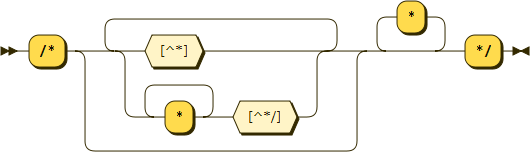
\includegraphics[scale=0.5]{kepek/rr_comment.png}
\caption{Comment}
\label{fig:rr_comment}
\end{figure}

\begin{figure}[h!]
\centering
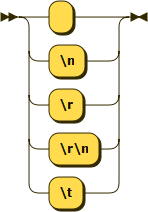
\includegraphics[scale=0.5]{kepek/rr_whitespace.png}
\caption{Whitespace}
\label{fig:rr_whitespace}
\end{figure}

\begin{figure}[h!]
\centering
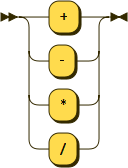
\includegraphics[scale=1]{kepek/rr_operator.png}
\caption{Operator}
\label{fig:rr_operator}
\end{figure}

\begin{figure}[h!]
\centering

\includegraphics[scale=1]{kepek/rr_digit.png}
\caption{Digit}
\label{fig:rr_digit}
\end{figure}

\begin{figure}[h!]
\centering
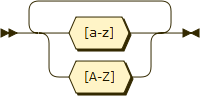
\includegraphics[scale=1]{kepek/rr_character.png}
\caption{Character}
\label{fig:rr_character}
\end{figure}

\begin{figure}[h!]
\centering
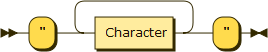
\includegraphics[scale=1]{kepek/rr_string.png}
\caption{String}
\label{fig:rr_string}
\end{figure}

\begin{figure}[h!]
\centering

\includegraphics[scale=1]{kepek/rr_block.png}
\caption{Block}
\label{fig:rr_block}
\end{figure}

\begin{figure}[h!]
\centering
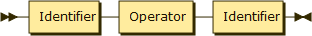
\includegraphics[scale=1]{kepek/rr_binaryoperator.png}
\caption{BinaryOperator}
\label{fig:rr_binaryoperator}
\end{figure}

\begin{figure}[h!]
\centering
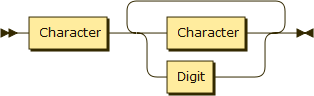
\includegraphics[scale=0.5]{kepek/rr_identifier.png}
\caption{Identifier}
\label{fig:rr_identifier}
\end{figure}

\begin{figure}[h!]
\centering
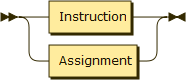
\includegraphics[scale=0.5]{kepek/rr_expression.png}
\caption{Expression}
\label{fig:rr_expression}
\end{figure}

\begin{figure}[h!]
\centering
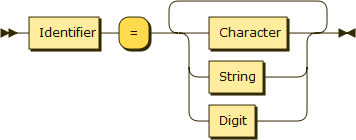
\includegraphics[scale=1]{kepek/rr_assignment.png}
\caption{Assignment}
\label{fig:rr_assignment}
\end{figure}

\begin{figure}[h!]
\centering
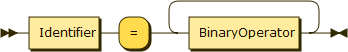
\includegraphics[scale=0.7]{kepek/rr_instruction.png}
\caption{Instruction}
\label{fig:rr_instruction}
\end{figure}

\begin{figure}[h!]
\centering
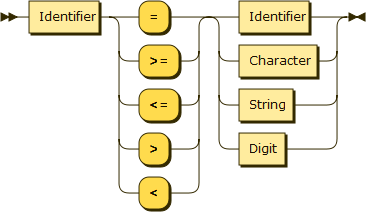
\includegraphics[scale=0.4]{kepek/rr_condition.png}
\caption{Condition}
\label{fig:rr_condition}
\end{figure}

\begin{figure}[h!]
\centering
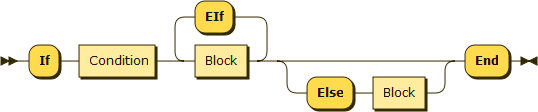
\includegraphics[scale=0.4]{kepek/rr_if.png}
\caption{If}
\label{fig:rr_if}
\end{figure}

\begin{figure}[h!]
\centering
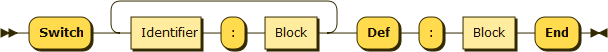
\includegraphics[scale=0.4]{kepek/rr_switch.png}
\caption{Switch}
\label{fig:rr_switch}
\end{figure}

\begin{figure}[h!]
\centering
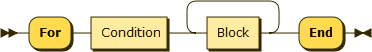
\includegraphics[scale=0.4]{kepek/rr_for.png}
\caption{For}
\label{fig:rr_for}
\end{figure}

\begin{figure}[h!]
\centering
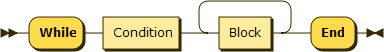
\includegraphics[scale=0.4]{kepek/rr_while.png}
\caption{While}
\label{fig:rr_while}
\end{figure}

\begin{figure}[h!]
\centering
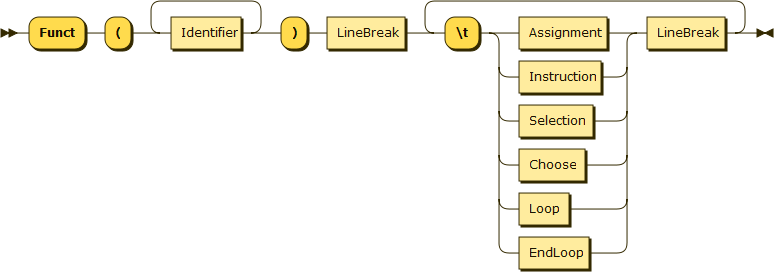
\includegraphics[scale=0.4]{kepek/rr_function.png}
\caption{Function}
\label{fig:rr_function}
\end{figure}

\begin{figure}[h!]
\centering
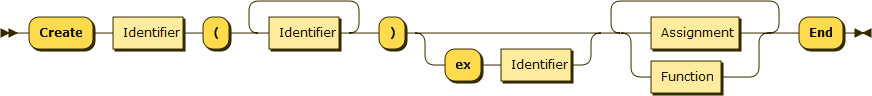
\includegraphics[scale=0.4]{kepek/rr_class.png}
\caption{Class}
\label{fig:rr_class}
\end{figure}

\begin{figure}[h!]
\centering

\includegraphics[scale=1]{kepek/rr_program.png}
\caption{Program}
\label{fig:rr_program}
\end{figure}

\section{Példák}

Az alábbiakban egy egyszerűbb példa forráskód részletet, melyben egy osztály és a benne lévő elemek láthatók.

\begin{verbatim}
Create Ember
	
	Ember(string nev, int kor, int irSzam, string utca, int hSz)
		string @nev = nev
		int @kor = kor
		Cim @cim = Cim(irSzam, utca, hSz)
	End
		
	Funct void @decrKor(int szam)
		While szam>0
			@kor = @kor - 1
			@szam = @szam --
		End
	End
	
	Funct string @createString()
		@nev + @kor + @cim.createString
	End
End
\end{verbatim}
		
Az alábbiakban a fenti osztály példányosítása és használatának példája látható

\begin{verbatim}
Ember pelda = Ember("teszt", 20, 1542, "Teszteles", 50)
pelda.setParam1("TesztKetto")
string ember = pelda.createString()
\end{verbatim}

\Chapter{Szintaktikai elemzés}

% TODO: Formális nyelvekkel, fordítóprogramokkal kapcsolatos könyvek hivatkozásai.

% http://www.informatik.uni-bremen.de/agbkb/lehre/ccfl/Material/ALSUdragonbook.pdf

\section{Java parser generátorok}

Az Interneten sokféle parser generátor található, mely segítségével a szintaktikai elemzés könnyebbé válik, megoldható.
A feladat megoldásához olyan parser generátorra van szükség, mely Java nyelvű, mivel a fordítóprogram ezen a nyelvek kerül megírása.
Emellett a parser generátorok feldolgozás szempontjából is sokfélék, és jelen feladathoz olyan generátort kellett keresni, mely reguláris nyelvvel képes működni.
Az alábbiakban a legelterjedtebb ilyen generátorokat vizsgáljuk meg.

\subsection{AnnoFlex}

Az Annoflex egy Java alapú generátor, mely szabadon letölthető és használható, sőt módosítható is. Az AnnoFlex implementálható mind az Eclipse, mind a InteliJ fejlesztőpi környezetekbe, külső eszközként, így bármikor használható lesz.

Az AnnoFlex megalkotáskor is a használata minél egyszerűbbé tétele volt a fő szempont, legegyszerűbb esetben az alábbi kódot kell megírnunk:

\begin{java}
/**
* @option methodName = getNextToken
* @option statistics = enabled
*/
public class Example_Annoflex {
/** @expr [0-9]+       */ String createNumber()     { return "number"; }
/** @expr [a-zA-Z]+    */ String createIdentifier() { return "identifier"; }
/** @expr [ \n\r\t\f]+ */ String createWhitespace() { return "whitespace"; }

//%%LEX-MAIN-START%%


//%%LEX-MAIN-END%%
}
\end{java}

Az AnnoFlexnek meg kell adni a beállításokat, méghozzá a megvalósítása szerint az osztálynév előtt és komment formájában kell megadni őket, valamint fontos, hogy a @option annotáció előzze meg őket. Példánkban a metódus nevét állítottuk be, illetve azt, hogy a generálás során statisztikát jelenítsen meg a program.

Ezután az osztályon belül meg kell adni a kifejezéseket és a metódusokat. Itt találkozhatunk több megkötéssel is az AnnoFlex tekintetében. A megadáskor mindenképpen @expr kifejezéssel kell kezdeni, melyet szintén kommentben kell elhelyezni.

A kifejezés után csak és kizárólag reguláris kifejezés állhat. A komment után magát a metódust kell megírni, melynél szintén van megkötés. A metódusok nem lehetnek static módosítóval ellátva, visszatérési értékük nem lehet csak primitív típus vagy String, de mindenképpen az összes így megadott metódusnak ugyanolyan visszatérési értékkel kell bírnia, egyetlen kivétellel, ami a void. Void visszatérési érték állhat más visszetérési érték mellett. További megkötés, hogy a metódusoknak nem lehet paraméterük, csak visszatérési értékük.

Minden egyes metódust csak egy darab reguláris kifejezés előzhet meg, ha több reguláris kifejezés is kellene, hogy ott álljon, akkor a reguláris kifejezések uniójával oldható ez meg, melyhez a | operátor használható.

Ez után következik egy tagek által határolt üres rész, ezt mindig a //%%LEX-MAIN-START%% és //%%LEX-MAIN-END%% határolja, és ide kerül legenerálásra a tulajdonképpeni kód. Ebben ad nagy segítséget az AnnoFlex.

Amennyiben elkészültünk a kifejezések megírásával, akkor a fejlesztőkörnyezetben lefuttathatjuk a AnnoFlex programot, mely eredménye a következő lesz:

% TODO: Itt csak behivatkozni majd valahogy a generált kódot, és csak néhány érdekesebb kódrészt mutatni belőle!

% TODO: Fel lehet sorolni a generált adattagokat és metódusokat!

A fenti kódban látható, hogy a program legenerálta a szükséges metódusokat és funkciókat. Ezután már nem kell mást tenni, mint egy futtatható osztályt készíteni a példához:

\begin{java}
public class Example_AnnoRun {

	public static void main(String[] args) {
		Example_Annoflex anno = new Example_Annoflex();
		anno.setString("Ez 1 teszt string");
		System.out.println("Scan:" + anno.getString());
		String token = anno.getNextToken();
		while (token != null) {
			System.out.println(token + ":" + anno.getMatchText());
			token = anno.getNextToken();
		}
	}

}
\end{java}

Ebben csak létrehozunk egy példányt az osztályból, hozzáadunk egy szöveget és lefuttatjuk a programot. A képernyőre a következő eredményt fogja a program kiírni:

\begin{verbatim}
Scan:Ez 1 teszt string
identifier:Ez
whitespace: 
number:1
whitespace: 
identifier:teszt
whitespace: 
identifier:string
\end{verbatim}

Látható, hogy identifier-nek jelezte a szövegeket, a számot numberként jelenítette meg és megtalálta a fehér karaktereket is, azaz a szóközöket.

\subsection{JFlex}

A JFlex szigorú értelembe véve egy lexikai elemző, azaz lexer generátor, mely Java nyelvhez Java nyelven írt generátor. Itt is a megadott inputot próbálja meg illeszteni a különféle előre definiált nyelvtani elemekre és az annak megfelelő utasításokat hajtja végre.

A JFlex a JLex átírt változata, melynek átírásakor a cél a teljes unicode támogatás és platformfüggetlenség volt, illetve a gyors szkenner generálás, kényelmes szintaktika és az is, hogy kompatibilis legyen a JLex-el. Önállóan is használható, de mivel főképp lexer generátor, így más parser generátorokkal történő együttműködésre tervezték, leginkább a CUP parserrel kompatibilis.

Felépítése alapján a nyelvtani specifikáció három részre osztható, melyeket a \texttt{\%\%} jel választ el. Az első a felhasználói kód, a második a beállítások és makrók része, míg a harmadik fogja tartalmazni a lexer szabályokat.

% TODO: Itt is csak említeni kellene a példával kapcsolatban néhány észrevételt!

\subsection{AustenX}

Az AustenX, vagy röviden csak Austen szinten egy parser generátor. Az Austen jelenleg csak Java nyelven nyújt generátort, és az előzőekhez hasonlóan ez is reguláris nyelv alapján dolgozza fel a kódot.

Az Austin egy jar fájlként tölthető le és futtatható, aminek futtatásakor paraméterként kell megadni a célfájlt. Az Austen futtatható a jar fájlra kattintva duplán, ilyenkor egy egyszerű felhasználói kezelőfelület nyílik meg. Itt meg kell adni a forrásfájlok helyét, amiben a feldolgozáshoz szükséges adatok vannak, illetve a célfájl helyét, ahova a feldolgozott fájlok kerülnek. A forrásfájlok .austen vagy .austenx kiterjesztéssel kell, hogy rendelkezzenek. Az alábbiakban egy egyszerűbb példa látható a forrásfájlokra.

% TODO: Tömören össze kellene foglalni a generált kódot.

A fenti kód egy általános leírást tartalmaz, library-k szerint szervezve melyet felhasznál az alábbi kód, ami a parser generator pontos leírását tartalmazza.

\Chapter{Közbülső reprezentáció}

A keresztfordító működése szerint beolvassa a nyelvi fájlt, melyet a programozó a definiált nyelven megírt, majd szekvenciálisan feldolgozza azt. A szinkatkikai elemzés után egy belső szerkezet jön létre, mely leírja a beolvasott programkódot.

A kód a belső szerkezetben osztályokba lesz szervezve, ezekről az alábbiakban kerül említésre néhány információ.

\begin{figure}
\centering
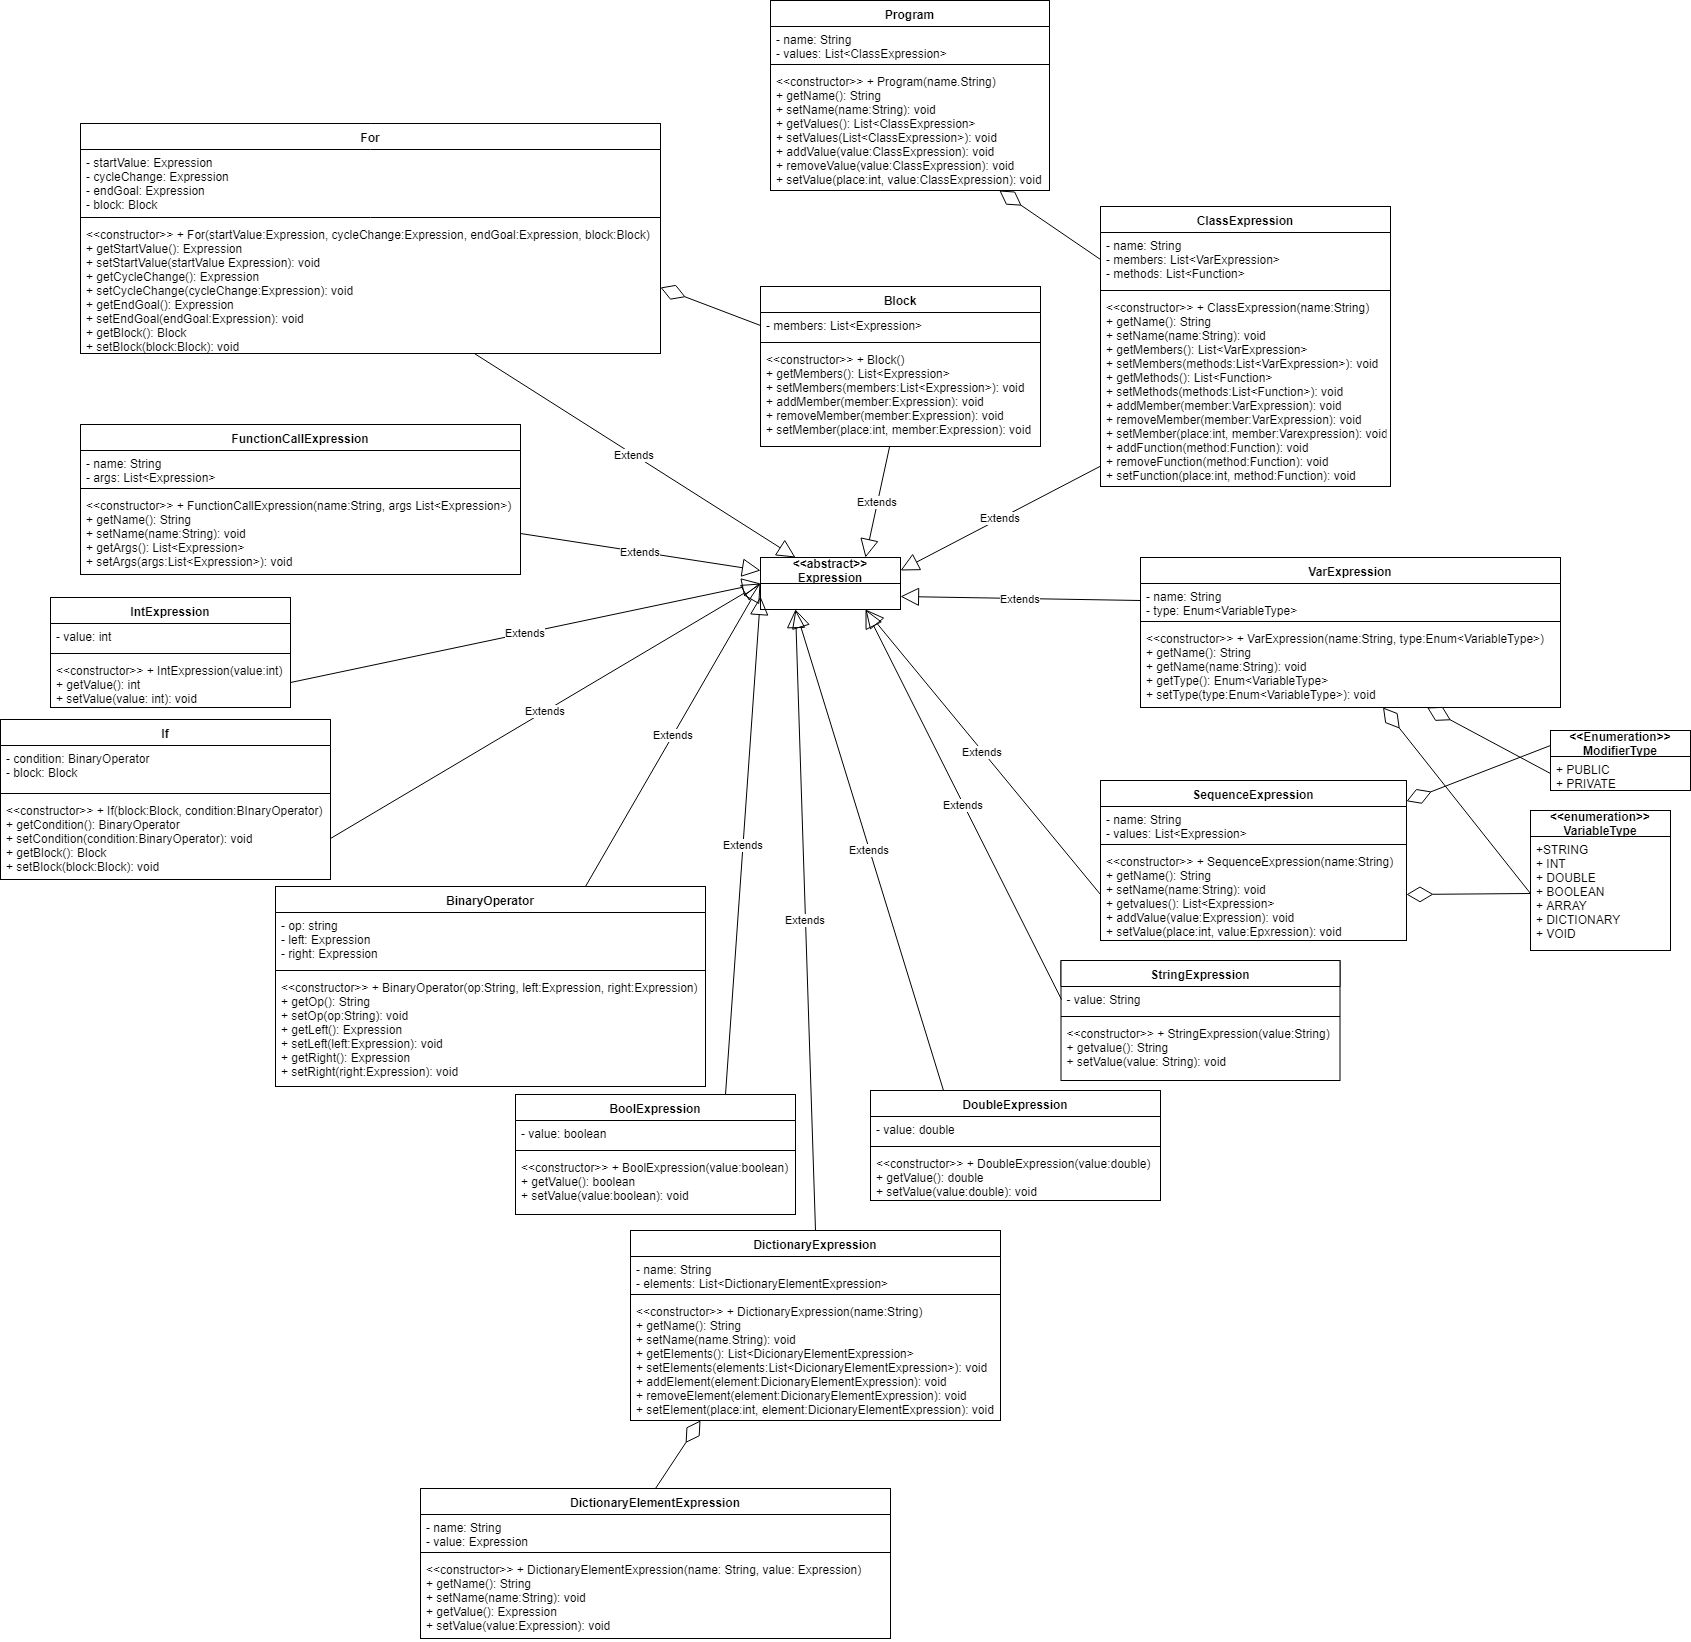
\includegraphics[scale=1]{kepek/rr_uml.png}
\caption{Osztálydiagram}
\label{fig:process}
\end{figure}

\begin{itemize}
\item függvénydefiníció
\begin{figure}
\centering
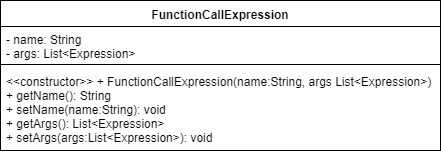
\includegraphics[scale=1]{kepek/rr_funccallexpr_dia.png}
\caption{Függvényhívás}
\label{fig:process}
\end{figure}
\item változó definíció
\begin{figure}
\centering
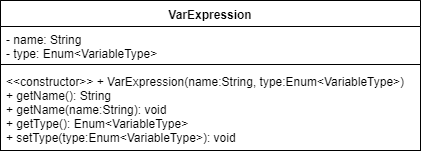
\includegraphics[scale=1]{kepek/rr_var_dia.png}
\caption{Változó osztály}
\label{fig:process}
\end{figure}
\item for ciklus
\begin{figure}
\centering
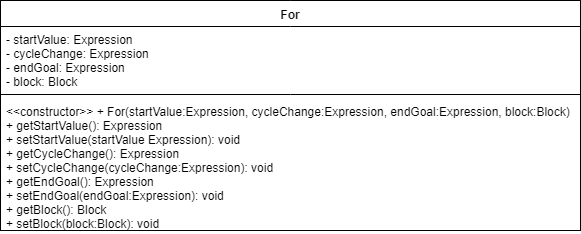
\includegraphics[scale=1]{kepek/rr_for_dia.png}
\caption{For ciklus osztálya}
\label{fig:process}
\end{figure}
\item feltételes elágazás
\begin{figure}
\centering
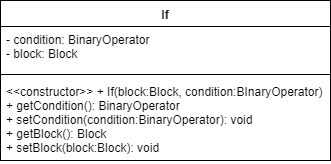
\includegraphics[scale=1]{kepek/rr_if_dia.png}
\caption{Feltételes elágazás, If osztálya}
\label{fig:process}
\end{figure}
\item osztály definíció
\begin{figure}
\centering
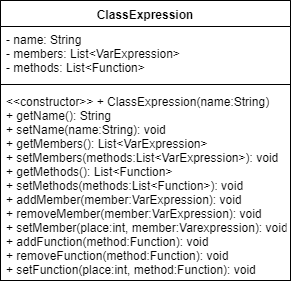
\includegraphics[scale=1]{kepek/rr_class_dia.png}
\caption{Osztály leírása osztályban}
\label{fig:process}
\end{figure}
\item program/modul/package definíció (befoglaló típusnak)
\begin{figure}
\centering
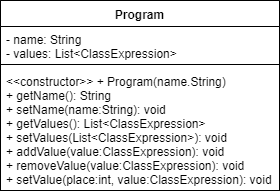
\includegraphics[scale=1]{kepek/rr_prog_dia.png}
\caption{Program osztály}
\label{fig:process}
\end{figure}
\item blokk/szekvencia típus
\begin{figure}
\centering
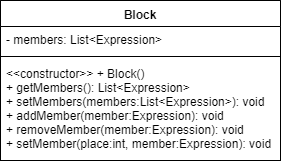
\includegraphics[scale=1]{kepek/rr_block_dia.png}
\caption{A keresztfordítás lépései}
\label{fig:process}
\end{figure}
\item expression/statement

\end{itemize}

% TODO: Jó sok UML diagram

% TODO: Absztrakt gyár mintát érdemes lesz majd bemutatni a kimeneti programnyelvek implementációjánál.

\Chapter{Célnyelvre fordítás}

Az alábbi részben a tervezett célnyelvek szintaxisának, elemeinek áttekintése történik meg a hangsúlyt az egyes célnyelvek különbözőségeire fektetve.

\section{Nyelvi típusok}

Az alábbiakban egy összefoglaló látható a különböző nyelvi típusokról, hogy az egyes célnyelvekben megjelenik-e az adott típus és ha igen akkor milyen formában. Ez alapján egy áttekintést kaphatunk arról, hogy a megírt kód lefordítása után az egyes nyelveket a típusok hogyan jelennek meg.
A kapott táblázat alapján meg tudjuk majd állapítani, hogy mely típusok jelennek meg a nyelvek nagy többségében, azaz a fordítás során mely típusokat kell mindenképpen figyelembe venni, megvalósítani.

Mivel a programozási nyelv megalkotása és a fordító megvalósítása során mindvégig a könnyű használhatóság és egyszerű megtanulhatóság lett szem előtt tartva, ezért jelen verzióban csak a fent említett közös típusok kerülnek megvalósításra. A későbbiekben ez bővíthető, hogy az egyes célnyelvek minden elemét tudja a program kezelni.

\begin{table}
	\caption{Programozási nyelvi típusok}
	\label{2. táblázat}
	\begin{tabular}{c|c|c|c|c}
		\textbf{C} & \textbf{Python} & \textbf{Java} & \textbf{JavaScript} & \textbf{PHP}\\
		char & - & - & string & string \\
		unsigned char & - & char & - & - \\
		signed char & - & - & - & A -> - \\
		int & int & int & number & integer \\
		unsigned int & - & - & - & - \\
		short & - & short & - & - \\
		unsigned short & - & - & - & - \\
		long & - & long & - & - \\
		unsigned long & - & - & - & - \\
		float & - & float & number & float vagy double \\
		double & inf & double & number & float vagy double \\
		long double & - & - & number & - \\
		void & - & void & - & - \\
		array & array & array & array & array \\
		pointer & - & - & - & - \\
		structure & class & class & object & object/class \\
		- & str & string & string & string \\
		- & boolean & boolean & boolean & boolean \\
	\end{tabular}
\end{table}

https://www.tutorialspoint.com/cprogramming/c\_data\_types.htm

https://realpython.com/python-data-types/

https://docs.oracle.com/javase/tutorial/java/nutsandbolts/datatypes.html

https://javascript.info/types

A táblázatból látható, hogy a C nyelvben alapvetően sok különféle típus került definiálásra, melyek a további nyelvekben vagy nem jelennek meg, vagy ha meg is jelennek, közös típus alá vannak rendelve, azaz egy-egy típust kell csak megjeleníteni a kódban.

Külön érdemes kiemelni a PHP, JavaScript és a Python nyelveket, melyeknél az egyszerű típusokat nem is kell megjeleníteni a kódban, az adott változó típusát mindig az aktuális értéke határozza meg. Bár igaz, hogy a típus az érték alapján kerül meghatározásra, ettől függetlenül az idézett dokumentációkban megjelennek az egyes típusok, hiszen a nyelvek a típusokat felismerik, függetlenül attól, hogy egy változó deklarálásakor meg kell-e adni azt vagy sem.

A fenti táblázat alapján a fordítóprogram a szám és szöveg típusú változókat támogatja, emellett a tömb, boolean és struktúra típust is. Jelenleg a további típusokat a fordítóprogram nem fogja támogatni, ezek beépítése egy további fejlesztési lehetőség lehet.

A szám típusok közül jelenleg az integer típus támogatott, mivel ez a leggyakrabban használt az általunk vizsgált témakörben, a szöveg string típusú lesz, mivel ez a megszokott a programozási nyelvek tekintetében, csakúgy mint a boolean típus. A definiált programozási nyelv típusosság tekintetében a Python nyelvre hasonlít, így a típus megjelölése itt sem szükséges.
A tömb típust itt dictionary néven fogjuk kezelni, a struktúra pedig a modern, objektum-orientált nyelvekhez hasonlóan osztályokból fog állni, melyek a változókat illetve függvényeket foglalhatnak magukba.

\section{Változók deklarálása}

Az alábbi részben áttekintjük, hogy az egyes célnyelvként tekintett magas szintű programozási nyelvekben a változó deklarálásában milyen különbségeket tapasztalhatunk. Az egyes célnyelvek függően attól, hogy a típusmegjelölést ki kell-e írni, illetve, hogy milyen kulcsszóval vagy kulcsszó nélkül adjuk meg az egyes változókat nagyban különböznek. Ezt a különbséget a fordítóprogramnak kezelnie kell, és el kell fednie a felhasználó elől.

A legfontosabb különbség a C és Java nyelv illetve a Python, JavaScript és PHP hármasa között van, ahogy a különbségek nagyobb részében így lesz. A változók deklarálása során az előbbi két nyelvben minden esetben ki kell írni a változó típusát a változó neve elé, például
\begin{cpp}
	int valtozo;
\end{cpp}

Azt is megtehetjük, hogy a deklarálással együtt inicializáljuk a változót, azaz egy értéket is adunk neki. Ez minden célnyelvként vett nyelv esetében működik, azaz megtehetjük, hogy az alábbi módon adjuk meg a változót például Java nyelven:

\begin{cpp}
	int valtozo = 12;
\end{cpp}

Ezzel szemben a Python, JavaScript és PHP nyelveken a típusmegjelölést nem kell kiírni a változó elé, viszont ezen nyelvek többségében is jelezni kell, hogy egy változót adunk meg.

A Python nyelvben kivételesen nem kötelező ezt megadni, sőt a korai Python verziók esetében több helyen is megjegyzik, hogy "nem szükséges a változókat deklarálni mielőtt használjuk őket, sőt a változók típusát sem kell megadni". (https://www.learnpython.org/en/Variables\_and\_Types)
Általánosságban ilyenkor annyit mondhatunk, hogy egy nevet rendelünk egy értékhez, hogy milyen típus lesz az, azt az érték fogja meghatározni.

\begin{cpp}
	valtozo = 12
	print(valtozo)
\end{cpp}

Ennek hátránya a nehézkes kódolvasás és javítás, főleg komplex programok esetén, mivel egy adott változó bármilyen típusú értéket felvehet, de lehetséges, hogy az adott változót használó kódrésznek egy adott típusú változóra lenne szüksége, ilyen esetben nehéz lehet megtalálni a probléma pontos forrását. Ennek kiküszöbölésére a 3.6-os Python verziótól kezdődően lehetőség van a egy úgynevezett "hint" megadására a változónevek után, melyben megadhatjuk, hogy terveink szerint az adott változó milyen típusú értéket fog felvenni.

\begin{cpp}
	valtozo: str = "szöveg"
	print(valtozo)
\end{cpp}

A Pythonhoz készített ellenőrzők, például a mypy program, már képesek ezeket feldolgozni, és a Java fejlesztőkörnyezethez hasonlóan kódoláskor már jelezni az esetleges típusbeli eltéréseket. Forrás: https://medium.com/@ageitgey/learn-how-to-use-static-type-checking-in-python-3-6-in-10-minutes-12c86d72677b

A JavaSript nyelvben ismét más megoldást vezettek be a változók esetében, itt a Java nyelvhez hasonlóan deklarálni kell a változókat, azonban típust itt sem kell megadnunk. A deklarálás mikéntjének vizsgálatában ismét először nézzük meg a régebbi verziókat először. Itt még csak a var kulcsszóval történik a deklaráció, és szokásos módon itt is azonnal értéket is tudunk adni a változónak.

\begin{cpp}
	var valtozo;
	valtozo = "szöveg";
	
	var valtozo2 = 12;
\end{cpp}

Az ilyen módon deklarált változók minden esetben az őket bezáró funkciókban érhetők csak el, illetve globálisan ha nincs bezáró funkció.
Az ECMAScript 2015 bevezetésekor változott ez meg, ami ECMAScript6 néven terjedt el a programozók körében. Ebben bevezettek két új váltózó típust és deklarálásukat.

\begin{cpp}
	let valtozo = "szöveg";
	
	const valtozo = "szöveg";
\end{cpp}

A let esetében, nem csak a bezáró funkcióban, de azon belül is csak abban a bezáró blokkban használható, ahol deklarálva lett.

\begin{cpp}
	var valtozo = 5;
	console.log(valtozo);
	{
		let valtozo = 8;
		console.log(valtozo);
	}
	console.log(valtozo);

\end{cpp}

A fenti példában az első konzol kiíratás 5-öt fog megjeleníteni, a második 8-at, míg a harmadik szintén 5-öt. Azonban fontos megjegyezni, hogy ha így írjuk meg a kódot

\begin{cpp}
	{
		let valtozo = 8;
		console.log(valtozo);
	}
	console.log(valtozo);
	
\end{cpp}

akkor a második kiíratás hibára fog futni, hiszen ahogy említettük, a let kulcsszóval deklarált változó csak az adott bezáró blokkon belül érhető el.

A const kulcsszóval deklarált változók majdnem teljesen úgy működnek, mint a let kulcsszóval deklaráltak, azaz csak az adott blokkon belül érhetők el, azonban ezek konstansok, azaz értékük nem változik.
Forrás: http://es6-features.org/#Constants, http://es6-features.org/#BlockScopedVariables, https://www.w3schools.com/js/js\_es6.asp, https://www.sitepoint.com/how-to-declare-variables-javascript/

A PHP nyelv ebből a szempontban nagyon egyszerű, itt sem kell típust kiírni, és a változó deklarálásakor a név előtt egy \textdollar jelet kell megadni.

\begin{cpp}
	$valtozo = 8;	
\end{cpp}

\section{Tömbök definiálása}

A tömböket általánosságban hasonlóan kell definiálni az egyes célnyelveken, de itt is okozhatnak nehézséget a fordítóprogram megvalósítása szempontjából a kisebb különbségek is.

A C nyelvben a tömbök deklarálásához meg kell adni először a tömb típusát, majd a nevét, végül a tömb méretét [ és ] között. A tömböt azonnal fel is tölthetjük elemekkel, ekkor nem kell a tömb méretét külön megadni, csak az egyenlőségjel után { és } jel között kell felsorolni a tömb elemeit.
Ha csak az egyik elemet akarjuk módosítani akkor a név után [ és ] jel között meg kell adni hanyadik elemet akarjuk módosítani majd az elem értékét. A tömb mindig a 0-ás indexelésű lesz, azaz az első elem a 0. indexű.

\begin{cpp}
	int tomb[10];
	int tomb2[] = {1, 5, 10, 25};
	int tomb[2] = 4;
\end{cpp}

A Java nyelv hasonlóan működik, azzal a különbséggel, hogy a tömbök típusa után kell megadni a szögletes zárójelpárt, és a méretét csak az inicializálás során kell megadni.

\begin{cpp}
	int[] tomb;
	tomb = new int[5];
	
	int[] tomb2 = new int[]{3, 5, 2};
\end{cpp}

A tombök tekintetében a JavaScript, PHP és Python elég hasonlóan működik. Mindhárom nyelv esetében meg kell adni a tömb nevét, ami egy váltzó lesz, majd felsorolni a tömb elemeit, melyek többféle típusúak is lehetnek. Az adott tömbök futás alatt bővíthetők, tehát új elemet hozzá lehet adni a tömbökhöz. Ez utóbbival vigyázni kell, mivel egy adott változó direkt módon egy adott helyre történő beillesztése a tömbbe akár lyukakat is hagyhat a tömbben.

JavaScript alatt az alábbi módon valósítható meg a tömb kezelése:

\begin{cpp}
	var tomb = ["egy", "ketto"];
	
	console.log(tomb[1]);
	
	tomb[2] = "harom"; //Nem ajánlott használat
	tomb.push("harom"); //A tömb végére illeszti az elemet
	
	consloe.log(tomb.length); //Tömb méretének lekérdezése
\end{cpp}

Ugyanez a tömbkezelés Python alatt:

\begin{cpp}
	tomb = ["egy", "ketto"];
	
	print(tomb[1]);
	
	tomb.append("harom"); //A tömb végére illeszti az elemet
	
	print(len(tomb)); //Tömb méretének lekérdezése
\end{cpp}

És végül a kezelés PHP alatt az alábbi lesz:

\begin{cpp}
	$tomb = array("egy", "ketto");
	
	echo $tomb[1];
	
	$tomb[2] = "harom"; //Nem ajánlott
	array_push($tomb, "harom"); //A tömb végére illeszti az elemet
	
	echo count($tomb); //Tömb méretének lekérdezése
\end{cpp}


\section{Ciklusok}

A célnyelvként tekintett programozás nyelvekben a ciklusok megvalósítása nagyon hasonlóan működik, minden tekintett célnyelvben van elöltesztelő és hátultesztelő ciklus is. A ciklusokban minden esetben van egy feltétel, egy ciklusváltozó, melynek változása lesz a feltétellel összehasonlítva és egy ciklusmag, mely minden iterációban lefut.

A fontos különbség a tekintett célnyelvek között, hogy maga a nyelv sajátosságai megtalálhatók itt is, tehát például a Python nyelvnél nincs a ciklusmag { és } közé téve, de természetesen függetlenül ettől ez is blokkot képez. A többi nyelvnél általában a kapcsos zárójel kiírásával megjelenítik a blokkot.

A ciklusoknak a két fajtája, a while és a for minden nyelvben megtalálható.

\begin{cpp}
	for (int i = 1; i < 10; i++) {
		System.out.println(i + "\n");
	}

	int j = 1;
	while (j < 10) {
		System.out.println(j + "\n");
		j++;
	}
\end{cpp}

A fenti példa egy Java kód a ciklusokra. A C nyelvben ez a ciklusszervezés majdnem teljesen megegyezik, a fő különbség az, hogy a C nyelvben a változókat mindig előre, a program elején kell deklarálni, tehát az nem tehető meg a ciklus fejlécében.

A Python while ciklusa azonos a fenti kódban írtakkal, természetesen a nyelvi sajátosságok miatt fennálló különbségek kivételével. A for ciklus ebben az esetben kicsit megváltozik, de így is hasonlít a Java nyelvben található foreach ciklusra, mivel ilyenkor egy listán fut végig a ciklus.

\begin{cpp}
	tomb = ["egy", "ketto", "harom"];
	for i in tomb:
		print(i)
\end{cpp}

JavaScript és PHP alatt a ciklusok majdnem teljesen megegyeznek a Java kódban látható ciklusokkal, természetesen itt is meg kell említeni a nyelvi sajátosságokat (pládul a PHP változók előtt itt is szerepelnie kell a \textdollar szimbólum), melyek eltéréseket okoznak és melyeket figyelembe kell venni a kimeneti kód megalkotásakor.

\section{Függvények}

A függvények kezelése a célnyelvekben szintén hasonlóan működik. A függvényeknek kell legyen egy fejlécük, melyben megadjuk a nevüket, visszatérési értékük típusát ahol kell, és a paraméter listát, illetve szükséges egy függvénytörzs is.

A fő különbség itt a C nyelvben van, ahol a függvényeket előre definiálni kell, egy prototípust kell a program elején írni belőlük, melyben fel kell tüntetni a függvény visszatérési értékének típusát, nevét és a paraméterek típusait. Ez a C nyelv esetében azért szükséges mivel a programnak tudnia kell a függvényről a meghívás helyén, és régebbi konvenció szerint a program belépési pontja azaz a main függvény után írjuk a többi függvényt. Azonban ha minden függvény teljesen megírásra kerül a main függvény előtt, függvényprototípusokat nem szükséges definiálni. Ezt kihasználva a C nyelvre fordítás is egyszerűsödhet a függvények kezelése szempontjából.

\begin{cpp}
	public static void main(String[] args) {
		int i = 1;
		int j = 2;
		System.out.println(addFunction(i,j));
	}
	
	public int addFunction(int a, int b) {
		return a+b;
	}
\end{cpp}

A fenti Java kódban egy függvényt és annak meghívását lehet látni. A függvények és meghívásaik a többi célnyelvként tekintett programozási nyelven is hasonlóan működnek.

A fő különbség a Python nyelven, hogy itt a nyelvi sajátosságok miatt általában nem kell láthatósági módosítót és visszatérési érték típust megadni, ellenben a def kulcsszóval kell a függvény leírását bevezetni. Meghívása a Java nyelvhez hasonlóan a függvény nevével történik. Ahogy a függvény neve elé nem kell, úgy a paraméterlistában a paraméterek nevei elé sem kell a típus megjelölés, azonban az újabb Python verziókban a fentebb említett "hint" itt is használható.

A PHP esetében a különbség majdnem ugyanaz, mint a Python esetében, tehát nem kell láthatósági módosító és típusmegjelölés sem, viszont a függvényt itt is kulcsszóval kell bevezetni, ez pedig a function lesz a PHP esetében. A paraméterek elő itt is kell a változóknál említett \textdollar szimbólum.

A JavaScript esetében szintén ez a helyzet mint az előző két esetben, és itt is a function kulcsszóval kell bevezetni a függvényt.

A függvények esetében visszatérési érték is lehetséges, hiszen a függvénytörzsben elvégzett adatokkal akár vissza is térhet a függvény a meghívó függvénybe. Ezt a return utasítással kell megadni minden nyelvben.

Szintén érdekesség, hogy a függvények paraméterének a legtöbb nyelvben lehet egy alapértelmezett értéket adni, és amennyiben nem kap értéket a meghíváskor, akkor ezt a kezdeti értéket fogja használni.
A C nyelv ebből a szempontból sajnos kivétel, nem támogatott alapértelmezetten ez a megoldás, természetesen különböző módokon lehet olyan programot írni melyben akár struktúrákkal, akár több függvénnyel a fent leírt hatás elérhető, de ez nehézkes. A legközelebbi beépített megoldás ezzel kapcsolatban a változó paraméterekkel (varargs) megoldott függvény lenne, de ez nem a legegyszerűbb megoldás és itt az ellenőrzések sem egyszerűek.
Ugyanígy a Java nyelv sem támogatja ezt a funkciót. Természetesen itt is megoldhatók ezek, itt a függvénytúlterhelés (function overloading) lenne a megoldás, amely esetben több függvényt írunk ugyanazon néven különböző paraméterlistával (ezt a Java támogatja), és az egyes függvények csak meghívják a további függvényeket melyek mind több és több paramétert tartalmaznak, míg végül az eredetileg megírni kívánt függvényt is. Az egyes függvények pedig a több paraméterrel rendelkező függvényeket egy alapértelmezett paraméterrel hívják meg, így a felhasználó mindig azt a függvényt tudja meghívni amennyi paraméter éppen a rendelkezésére áll a többi pedig alapértelmezett értékekkel kerül kitöltésre. Sajnos a nagyobb függvények esetében ez is eléggé bonyolulttá teszi nem csak a kódot de az ellenőrzést és javítást is.

A JavaScript a ECMAScript 2015-től kezdődően támogatja az alapértelmezett paramétert, csakúgy mint a PHP és a Python is támogatja ezt, így ez a három célnyelv az ami a kód bonyolítása nélkül képes ezeket kezelni.

Minthogy két nyelv is van a célnyelvként választott nyelvek között mely ezt nem támogatja, ezért a rugalmasságot és egyszerűséget alapul véve a definiált nyelvben sem lesz egyenlőre ez a funkció benne, így alapértelmezett paramétereket nem tudnak a felhasználók megadni. A fordítóprogram további fejlesztésekor, a felhasználói visszajelzéseket figyelembe véve lehet kibővíteni ezzel a rendszert.

\section{Struktúra és osztály}

Általánosságban a kódot a célnyelvekben valamilyen struktúrába szervezik. A magas szintű, modern programozási nyelvek az osztályokba szervezést követik, azaz a kódot valamilyen szempont alapján különböző osztályokba szervezik és ezek együttműködnek a program futása során.

A dolgozat szempontjából célnyelvként vizsgált nyelvek szinte mindegyike támogatja az osztályokba szervezést, kivéve a C nyelvet, melyben máshogy lehet ehhez hasonló szerkezetet megoldani.

\begin{cpp}
	public class Osztaly {
		int a;
		
		public Osztaly(int a) {
			this.a = a;
		}
	
		public int getA() {
			return this.a;
		}
	}
\end{cpp}

A fenti rövid Java nyelven írt példa mutatja be az osztályokat. A vizsgált célnyelvek közül a C nyelvet kivéve az osztályok megalkotása ehhez hasonlóan működik, minden osztálynak kell egy neve legyen, adattagjai és metódusai. Java nyelven az osztálynak egy láthatósági módosítója is van. Az adott nyelveken az osztályoknak van egy kiemelt metódusuk, a konstruktor. A Java nyelven ez az osztály nevével ellátott függvény lesz, melynek nincs visszatérési értéke, ez inicializálja a változókat, melyeket osztályon belül adattagnak nevezünk. Java nyelven lehetőség van több konstruktort is írni a fentebb említett method overloading segítségével, így egy osztály többféle módon is példányosítható lesz.
A példányosítás után az egyes metódusokra (amennyiben elérhetőek) a . operátorral hivatkozhatunk.

JavaScript nyelven az osztály tulajdonképpen egy egyedi függvényként is tekinthető, azaz a megírt tartalom függvényként is definiálható lenne. Azonban az osztályban történő definiálás az áttekinthetőség és az egyszerűbb leírás miatt történt. JavaScriptben is a class kulcsszóval kell bevezetni az osztálydefiníciót, azonban láthatósági módosítót nem kell megadni hozzá. Itt is létezik konstruktor függvény, de itt a constructor néven kell megírni, és csak egy darab lehet belőle. A példányosítás után itt is a . operátorral hivatkozhatunk az osztály metódusaira, adattagjaira.

PHP nyelven szintén a class kulcsszóval kell bevezetni az osztály deklarálását, viszont itt különbség, hogy a konstruktort a \_\_constuct függvény néven kell megírni. Az osztály metódusaira és adattagjaira viszont itt a -> operátorral lehet hivatkozni.

A Python nyelven az előzőekhez hasonlóan szintén class kulcsszóval kell az osztályt létrehozni, viszont itt is másik néven szerepel a konstruktor, itt az \_\_init\_\_ függvényt kell megírni, melyet a nyelvi sajátosságok alapján a def kulcsszóval kell bevezetni. A metódusokra és adattagokra itt is a . operátorral lehet hivatkozni.

Ahogy fentebb említésre került, a C nyelv nem obejtum orientált nyelv, azaz osztályokat nem lehet definiálni, ezért ilyen esetben kerülő megoldás kell. A C nyelvben definiálhatunk struktúrákat, azonban itt problémát jelenthet, hogy a metódusokat nem tudjuk magában a struktúrában definiálni, azaz külön kell azokat definiálni és explicit átadni neki magát a struktúrát, hogy az adattagjait kezelni lehessen. Emiatt a program eléggé bonyolulttá válhat, könnyen összekeverhető, hogy melyik struktúrához mely függvények tartoznak. Ennek kivédésére különböző névkonvenciókat alkalmazhatunk. Viszont jelen dolgozat esetében nem kell a felhasználónak ilyennel foglalkoznia, hiszen a definiált nyelven megírt kódot a program fordítja le, így az állítja össze a célnyelvi megfelelőjét. Viszont sajnos ilyenkor ha a kimeneti programot tovább szeretné a felhasználó szerkeszteni akkor az nehézségeket okozhat, de mivel a bemeneti programot lehet a továbbiakban is szerkeszteni ezért a kimeneti fájlt nem szükséges szerkeszteni.
Az alábbiakban látható egy példa a C nyelven megírt osztályhoz hasonló program megvalósításra.

\begin{cpp}
	typedef struct osztalyDef {
		int a;
		int b;
	} osztaly;
	
	int osztaly_getA(osztaly* osztPeldany) {
		return osztPeldany->a;
	}
	
	int osztaly_getB(osztaly* osztPeldany) {
		return osztPeldany->b;
	}
	
	void osztaly_setA(osztaly* osztPeldany, int x) {
		osztPeldany->a = x;
	}
	
	void osztaly_setB(osztaly* osztPeldany, int x) {
		osztPeldany->b = x;
	}
	
	int osztaly_addNumber(osztaly* osztPeldany) {
		return osztPeldany->a + osztPeldany->b;
	}
	
	osztaly osztDef;
	
	int main()
	{
		osztaly_setA(&osztDef, 10);
		osztaly_setB(&osztDef, 5);
		
		printf("%d", osztaly_addNumber(&osztDef));
		
		return 0;
	}
\end{cpp}
\Chapter{Eredmények értékelése}

Ki kellene választani majd 5-10 algoritmust, amelyikhez egy-egy szakaszban szerepelnek az implementációk, utána pedig az egyes nyelvekre való fordítással kapcsolatos észrevételek, futási idők.


\Chapter{CD-melléklet tartalma}

A szakdolgozatom mellé egy darab CD tartozik, amely a következő adatokat tartalmazza $\ldots$


\begin{thebibliography}{x}
\addcontentsline{toc}{chapter}{\bibname}

Principles of Compiler Design

Formális nyelvek és automaták

\end{thebibliography}


\pagestyle{empty}
\vspace*{1cm}  
\begin{center}
\large\textsc{\bfseries Eredetiségi Nyilatkozat}
\end{center}
\vspace*{2cm}  

Alulírott \textbf{Horváth Máté János}; Neptun-kód: \texttt{U7C73N} a Miskolci Egyetem Gépészmérnöki és Informatikai Karának végzõs gazdasági informatikus szakos hallgatója ezennel büntetõjogi és fegyelmi felelõsségem tudatában nyilatkozom és aláírásommal igazolom, hogy
\textit{Programozási nyelv magas szinten átvihető alkalmazások fejlesztéséhez}
címû szakdolgozatom/diplomatervem saját, önálló munkám; az abban hivatkozott szakirodalom
felhasználása a forráskezelés szabályai szerint történt.\\

Tudomásul veszem, hogy szakdolgozat esetén plágiumnak számít:
\begin{itemize}
\item szószerinti idézet közlése idézõjel és hivatkozás megjelölése nélkül;
\item tartalmi idézet hivatkozás megjelölése nélkül;
\item más publikált gondolatainak saját gondolatként való feltüntetése.
\end{itemize}

Alulírott kijelentem, hogy a plágium fogalmát megismertem, és tudomásul veszem, hogy
plágium esetén szakdolgozatom visszautasításra kerül.

\vspace*{3cm}

\noindent Miskolc, \hbox to 2cm{\dotfill} év \hbox to 2cm{\dotfill} hó \hbox to 2cm{\dotfill} nap

\vspace*{3cm}

\hspace*{8cm}\begin{tabular}{c}
\hbox to 6cm{\dotfill}\\
Hallgató
\end{tabular}


\end{document}
